\mbox{}
\subsection{Modélisation UML}
A partir de l'analyse initiale ainsi qu'avec les informations obtenues à l'aide du diagramme des use-case et du diagramme d'activité, nous avons pu établir un premier diagramme de classe. Ce diagramme de classe, aussi appelé UML, représente un schéma des différentes entités (futurs tables) principales que nous allons retrouver plus tard dans la base de données. Nous pouvons aussi y trouver les associations nommées entre ces entités, et les cardinalités associées. Le logiciel que nous avons utilisé ne nous permettant pas d'autres cardinalités que 1 ou *, 1 vaut pour 1-1 et 0-1, tandis que * vaut pour 1-N et 0-N.\\

Le diagramme UML nous permet également de visualiser les fonctions nécessaires au bon fonctionnement du système d'informations. Dans le cas du diagramme que nous présentons à la page suivante, les fonctions définies sont les premières auxquelles nous avons pensé. Nous aurions du compléter ce diagramme à l'aide des fonctionnalités découvertes à l'aide des diagrammes de séquences, définis à la prochaine section. Cependant, nous avons manqué de temps, et nous n'avons pas su terminer les diagrammes de séquence. De ce fait, nous avons délibérément choisi de montrer le diagramme UML défini auparavant, ceci pour éviter d'avoir quelque chose de mal balancé dans nos classes.\\

 L'UML se trouve à la page suivante (p.\pageref{fig:uml}), figure \ref{fig:uml}.


\newpage
\begin{landscape}
\begin{figure}[H]
\centering
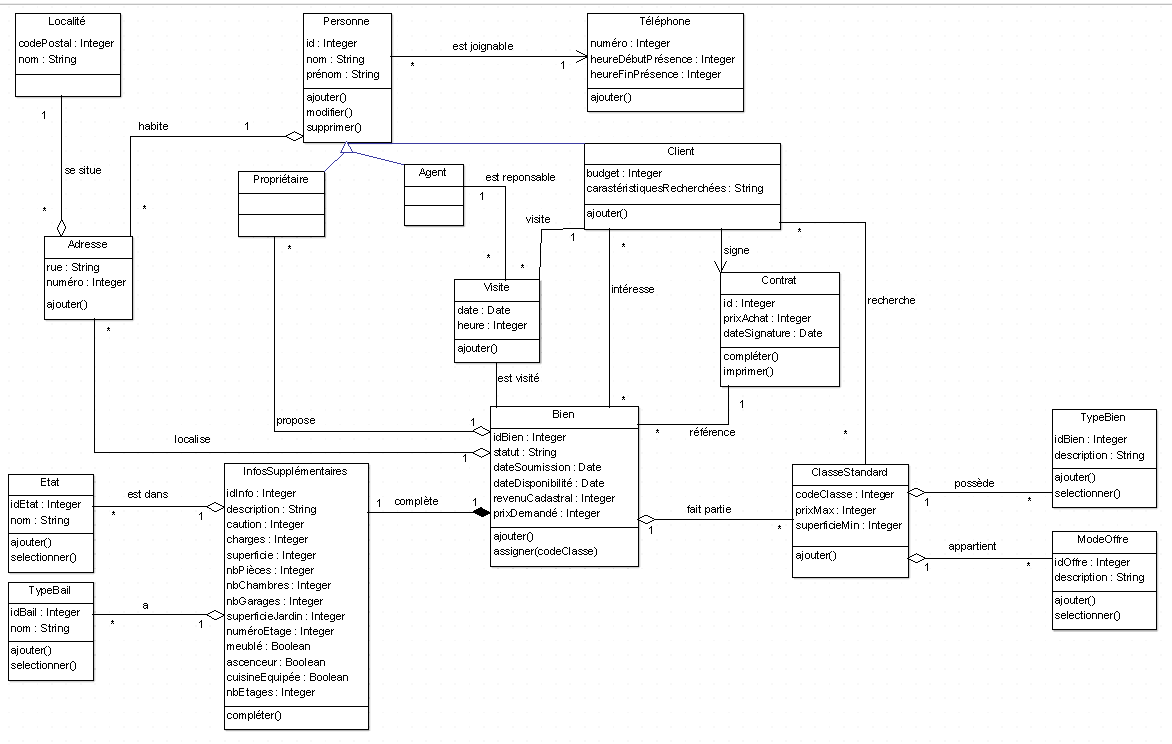
\includegraphics[width=23cm]{uml.png}
\caption{UML sur base des résultat des analyses précédentes.}
\label{fig:uml}
\end{figure}
\end{landscape}